\chapter{Mathematical Modelling of the Battlefield}
\label{ch:modelling}
This thesis aims to be innovative in 2 ways:
\begin{enumerate}
    \item Create a mathematical model of the battlefield.
     \item Asses whether state-of-the-art MARL techniques are able to develop interesting strategies in the framework of this model.
\end{enumerate}
This chapter will develop the first point.\\
The goal of a mathematical - or algorithmic - model is twofold:
\begin{enumerate}
    \item Make explicit which simplifications we'll make, both about the terrain itself as about the agents that interact on this terrain.
    \item Allow a computer to manipulate the model and simulate different situations and predict their outcomes.
\end{enumerate}
An important question is which level of detail we aspire to. As in all simulations, this must be a trade-off between making something as simple as possible to reduce computational complexity, and retain enough details to make it realistic and useful. To works towards this equilibrium, several versions of the model are developed with increasing levels of complexity.\\
All forms of the game subscribe to the multi-agent formalism for Markov games, as defined in section \ref{sec:intro_marl}.

%---------------------------------------------------------------------------------------
\section{First Model}
\label{sec:first_model}
Two opposing players, $P_0$ and $P_1$, each command two agents, which we'll consider to be tanks. The game is played on a flat terrain without obstacles. The  size of the game board is small, typically $7$x$7$ or $11$x$11$.\\

This game offers perfectly symmetrical capacities to both teams: every tank $T_i$ is the same and has following individual state vector $s^i_t$:
\begin{enumerate}
    \item a position $(x,y)$ on the board,
    \item a boolean value {\tt alive} that determines whether the agent in question is still alive,
    \item an integer {\tt ammo} that specifies how many shots an agent has left,
    \item an integer {\tt aim} that specifies whether the agent is aiming at one of the opposing agents.
\end{enumerate}
The global state $\bm{s_t}$ is then a tuple $(s_t^0, s_t^1, s_t^2, s_t^3) \in \bm{S}$ with $\bm{S}$ the set of global states.\\
Each agent can choose among $8$ actions:
\begin{enumerate}
    \item {\tt do\_nothing}\\
        As the name says, the agent does nothing and it's state vector $s^i$ doesn't change.
    \item {\tt aim0} \\
        Aims at the first tank of the opposing player and thus changes the {\tt aim} variable of it's state vector. The agent must be alive to be able to execute this action.
    \item {\tt aim1} \\
        Idem as above but aiming at the second tank of the opposing player.
    \item {\tt fire} \\
        Fire at the tank the agent is aiming at. This decreases the {\tt ammo} counter. The agent must be alive, have sufficient ammo and must be aiming before executing this action.\\
        If the opposing tank is in range (determined by a parameter {\tt max\_range}), it's {\tt alive} indicator will be set to {\tt False}. This means that every shot will result in a killed opponent if in range.
    \item 4 {\tt move} actions ({\tt north}, {\tt south}, {\tt east}, {\tt west})\\
        The agent will move one step in the desired direction, unless he will drop of the board or tries to move to a tile occupied by an other agent.
        %or comes too close to another agent\footnote{This is done to avoid that two agents will end up in the same spot since actions are, in the general case, executed simultaneously and if agents are too close, they can move to the same square.}.
\end{enumerate}

The joint action space $\mathcal{A}$ thus consists of all tuples of actions $(a_t^0, a_t^1, a_t^2, a_t^3)$ whereby the first two actions are executed by agents belonging to player $P_0$ and the two others by agents of $P_1$. Actions are executed simultaneously. A player loses when both his tanks are dead or out of ammo. While the out-of-ammo criterion is a realistic assumption, it also avoids long games without end and thus speeds up learning. Additionally, a small penalty is introduced for every step an agent takes. This should induce an agent to prefer shorter episodes. Experience has shown that this addition does indeed shorten the average game time and speeds up learning compared to no penalty. Additionally, at the reset of a game, all agents are placed in the same initial position.\\
All agents receive an observation from the environment that is based on the global state vector. An observation $o^i_t$ for agent $i$ consists of the following information:
\begin{itemize}
    \item His own position, remaining ammo and, if applicable, the opposing agent he is aiming at.
    \item The relative position of his team mate and of the opposing agents, if they are still alive.
\end{itemize}
This implies that an agent does not know the ammo situation of other agents nor if opposing agents are aiming. This is a design choice to mimic a realistic situation.\\

Figure \ref{fig:game_visual} shows the standard visualization of the game, where tanks of the blue player $P_1$ are both dead (since they are "greyed out").

\begin{figure}[htp]
    \centering
    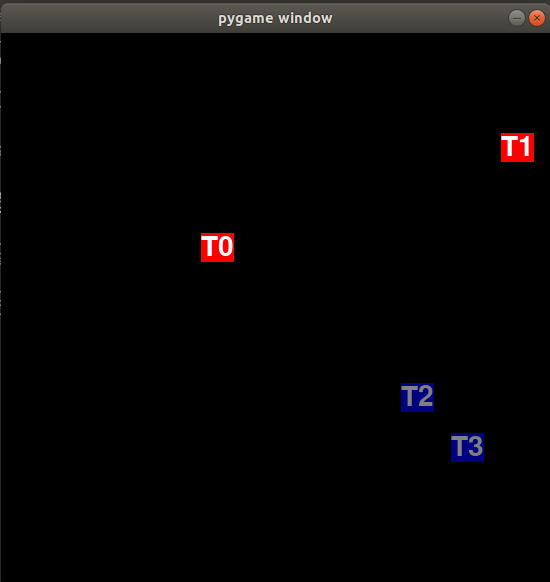
\includegraphics[width=8cm]{images/game_visual.png}
    \caption{Visualization of the simple version of the game}
    \label{fig:game_visual}
\end{figure}



%---------------------------------------------------------------------------------------
\section{Second Model}
The goal of extending the model is to make it more realistic. Several extension to the simple model have been considered. These proposed extension include:
\begin{enumerate}
    \item Using asymmetric agents with different capabilities (e.g. tanks vs. warriors with RPG)
    \item More than 2x2 agents
    \item Complex terrain where both visibility and mobility are blocked by obstacles.
    \item Larger state space, where e.g. fuel is limited.
    \item More complex firing probability, e.g. an exponentially decreasing probability based on distance between shooter and target.
\end{enumerate}
Since time was limited, only the second and third option were retained; the others will be explored in future research. This means that the second model is a model where the agent all have the same capabilities but the number of agents can be freely chosen. Furthermore, the terrain consists of free space and obstacles that block both the movement and the line-of-sight of the agents. A blocked line-of-sight means that firing is not allowed.\\
Just as before, each agent receives an observation from the environment which is derived from the global state. In this case, the agent receives:
\begin{itemize}
    \item His own position, ammo and aim
    \item The relative position of the other agents
\end{itemize}
such as before in the simple model. This observation is extended with information about which enemy agent is visible and can thus be fired at. This means that the agents don't receive information about the terrain directly; the only consequence of the terrain is implicitly captured in this visibility information. Adding more terrain information will be part of future research.

%%%
\textbf{TO DO}: discuss:
\begin{itemize}
    \item Sparse rewards
    \item Delayed rewards
    \item Credit assignment among agents
\end{itemize}